\documentclass[twoside]{article}\usepackage[]{graphicx}\usepackage[]{color}
% maxwidth is the original width if it is less than linewidth
% otherwise use linewidth (to make sure the graphics do not exceed the margin)
\makeatletter
\def\maxwidth{ %
  \ifdim\Gin@nat@width>\linewidth
    \linewidth
  \else
    \Gin@nat@width
  \fi
}
\makeatother

\definecolor{fgcolor}{rgb}{0.345, 0.345, 0.345}
\newcommand{\hlnum}[1]{\textcolor[rgb]{0.686,0.059,0.569}{#1}}%
\newcommand{\hlstr}[1]{\textcolor[rgb]{0.192,0.494,0.8}{#1}}%
\newcommand{\hlcom}[1]{\textcolor[rgb]{0.678,0.584,0.686}{\textit{#1}}}%
\newcommand{\hlopt}[1]{\textcolor[rgb]{0,0,0}{#1}}%
\newcommand{\hlstd}[1]{\textcolor[rgb]{0.345,0.345,0.345}{#1}}%
\newcommand{\hlkwa}[1]{\textcolor[rgb]{0.161,0.373,0.58}{\textbf{#1}}}%
\newcommand{\hlkwb}[1]{\textcolor[rgb]{0.69,0.353,0.396}{#1}}%
\newcommand{\hlkwc}[1]{\textcolor[rgb]{0.333,0.667,0.333}{#1}}%
\newcommand{\hlkwd}[1]{\textcolor[rgb]{0.737,0.353,0.396}{\textbf{#1}}}%
\let\hlipl\hlkwb

\usepackage{framed}
\makeatletter
\newenvironment{kframe}{%
 \def\at@end@of@kframe{}%
 \ifinner\ifhmode%
  \def\at@end@of@kframe{\end{minipage}}%
  \begin{minipage}{\columnwidth}%
 \fi\fi%
 \def\FrameCommand##1{\hskip\@totalleftmargin \hskip-\fboxsep
 \colorbox{shadecolor}{##1}\hskip-\fboxsep
     % There is no \\@totalrightmargin, so:
     \hskip-\linewidth \hskip-\@totalleftmargin \hskip\columnwidth}%
 \MakeFramed {\advance\hsize-\width
   \@totalleftmargin\z@ \linewidth\hsize
   \@setminipage}}%
 {\par\unskip\endMakeFramed%
 \at@end@of@kframe}
\makeatother

\definecolor{shadecolor}{rgb}{.97, .97, .97}
\definecolor{messagecolor}{rgb}{0, 0, 0}
\definecolor{warningcolor}{rgb}{1, 0, 1}
\definecolor{errorcolor}{rgb}{1, 0, 0}
\newenvironment{knitrout}{}{} % an empty environment to be redefined in TeX

\usepackage{alltt}
\usepackage[utf8]{inputenc}
\usepackage[czech]{babel}
\usepackage{fancyhdr}
\usepackage{amsmath}
\usepackage{amsfonts}
\usepackage[paper=a4paper, nomarginpar, foot=1.5cm, top=2.5cm, bottom=2.5cm, left=2.5cm, right=2.5cm]{geometry}
\usepackage{siunitx}

\pagestyle{fancy}
\fancyhead{} % clear all header fields
\fancyhead[RO,LE]{Marek Földi}
\fancyhead[RE,LO]{Úkol 4}
\fancyfoot{} % clear all footer fields
\fancyfoot[LE,RO]{\thepage}

\addto\captioneurosyfilisczech{\renewcommand{\figurename}{Graf. č.}}
\IfFileExists{upquote.sty}{\usepackage{upquote}}{}
\begin{document}





\subsection*{Příklad 1:}
\begin{knitrout}
\definecolor{shadecolor}{rgb}{0.969, 0.969, 0.969}\color{fgcolor}\begin{kframe}
\begin{alltt}
\hlstd{mod1} \hlkwb{<-} \hlkwd{aov}\hlstd{(loglym} \hlopt{~} \hlstd{infekt,} \hlkwc{data}\hlstd{=lymfo)}
\hlkwd{summary}\hlstd{(mod1)}
\end{alltt}
\begin{verbatim}
##              Df Sum Sq Mean Sq F value   Pr(>F)    
## infekt        4  54.85  13.712   10.65 9.88e-08 ***
## Residuals   171 220.10   1.287                     
## ---
## Signif. codes:  0 '***' 0.001 '**' 0.01 '*' 0.05 '.' 0.1 ' ' 1
\end{verbatim}
\begin{alltt}
\hlkwd{with}\hlstd{(lymfo,} \hlkwd{numSummary}\hlstd{(loglym,} \hlkwc{groups}\hlstd{=infekt,} \hlkwc{statistics}\hlstd{=}\hlkwd{c}\hlstd{(}\hlstr{"mean"}\hlstd{,} \hlstr{"sd"}\hlstd{)))}
\end{alltt}
\begin{verbatim}
##        mean        sd data:n
## EV 4.398098 1.2333843     45
## HV 5.167492 1.3598121     23
## KE 4.141498 0.9084437     46
## NB 4.498643 1.1620989     47
## NS 2.790502 0.9721319     15
\end{verbatim}
\begin{alltt}
\hlkwd{local}\hlstd{(\{}
  \hlstd{.Pairs} \hlkwb{<-} \hlkwd{glht}\hlstd{(mod1,} \hlkwc{linfct} \hlstd{=} \hlkwd{mcp}\hlstd{(}\hlkwc{infekt} \hlstd{=} \hlstr{"Tukey"}\hlstd{))}
  \hlkwd{print}\hlstd{(}\hlkwd{summary}\hlstd{(.Pairs))} \hlcom{# pairwise tests}
  \hlkwd{print}\hlstd{(}\hlkwd{confint}\hlstd{(.Pairs,} \hlkwc{level}\hlstd{=}\hlnum{0.95}\hlstd{))} \hlcom{# confidence intervals}
  \hlkwd{print}\hlstd{(}\hlkwd{cld}\hlstd{(.Pairs,} \hlkwc{level}\hlstd{=}\hlnum{0.05}\hlstd{))} \hlcom{# compact letter display}
  \hlstd{old.oma} \hlkwb{<-} \hlkwd{par}\hlstd{(}\hlkwc{oma}\hlstd{=}\hlkwd{c}\hlstd{(}\hlnum{0}\hlstd{,} \hlnum{5}\hlstd{,} \hlnum{0}\hlstd{,} \hlnum{0}\hlstd{))}
  \hlkwd{plot}\hlstd{(}\hlkwd{confint}\hlstd{(.Pairs))}
  \hlkwd{par}\hlstd{(old.oma)}
\hlstd{\})}
\end{alltt}
\begin{verbatim}
## 
## 	 Simultaneous Tests for General Linear Hypotheses
## 
## Multiple Comparisons of Means: Tukey Contrasts
## 
## 
## Fit: aov(formula = loglym ~ infekt, data = lymfo)
## 
## Linear Hypotheses:
##              Estimate Std. Error t value Pr(>|t|)    
## HV - EV == 0   0.7694     0.2908   2.646  0.06445 .  
## KE - EV == 0  -0.2566     0.2379  -1.079  0.81270    
## NB - EV == 0   0.1005     0.2366   0.425  0.99290    
## NS - EV == 0  -1.6076     0.3383  -4.753  < 0.001 ***
## KE - HV == 0  -1.0260     0.2897  -3.541  0.00448 ** 
## NB - HV == 0  -0.6688     0.2887  -2.317  0.14025    
## NS - HV == 0  -2.3770     0.3765  -6.313  < 0.001 ***
## NB - KE == 0   0.3571     0.2353   1.518  0.54484    
## NS - KE == 0  -1.3510     0.3373  -4.005  < 0.001 ***
## NS - NB == 0  -1.7081     0.3364  -5.077  < 0.001 ***
## ---
## Signif. codes:  0 '***' 0.001 '**' 0.01 '*' 0.05 '.' 0.1 ' ' 1
## (Adjusted p values reported -- single-step method)
## 
## 
## 	 Simultaneous Confidence Intervals
## 
## Multiple Comparisons of Means: Tukey Contrasts
## 
## 
## Fit: aov(formula = loglym ~ infekt, data = lymfo)
## 
## Quantile = 2.7435
## 95% family-wise confidence level
##  
## 
## Linear Hypotheses:
##              Estimate lwr      upr     
## HV - EV == 0  0.76939 -0.02842  1.56721
## KE - EV == 0 -0.25660 -0.90921  0.39601
## NB - EV == 0  0.10054 -0.54862  0.74971
## NS - EV == 0 -1.60760 -2.53558 -0.67961
## KE - HV == 0 -1.02599 -1.82087 -0.23112
## NB - HV == 0 -0.66885 -1.46090  0.12320
## NS - HV == 0 -2.37699 -3.40998 -1.34400
## NB - KE == 0  0.35714 -0.28841  1.00269
## NS - KE == 0 -1.35100 -2.27645 -0.42554
## NS - NB == 0 -1.70814 -2.63117 -0.78511
## 
##   EV   HV   KE   NB   NS 
## "bc"  "c"  "b" "bc"  "a"
\end{verbatim}
\end{kframe}
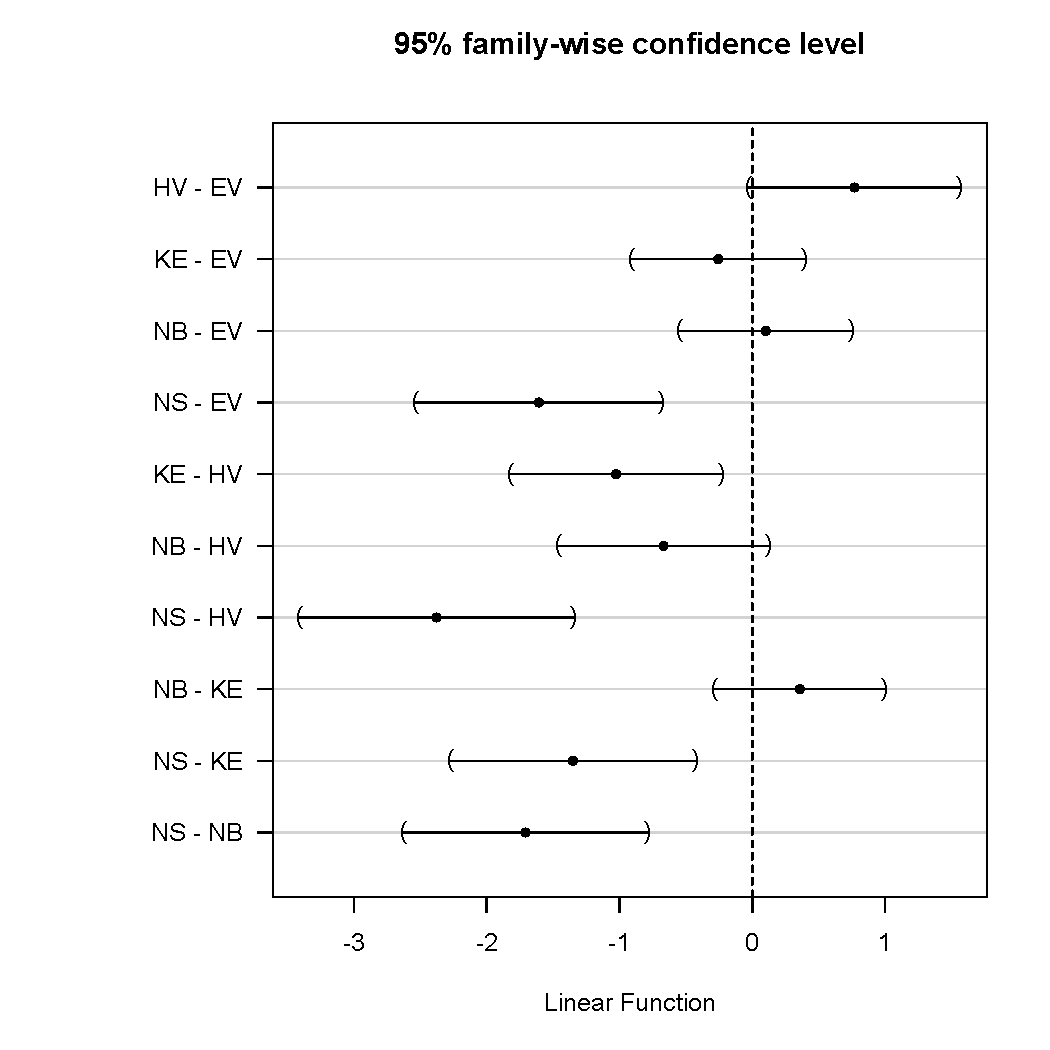
\includegraphics[width=\maxwidth]{figure/pr1-1} 

\end{knitrout}
Jelikož hodnota $\text{Pr}(>\text{F})$ je menší než 0,001 usuzujeme že mezi hodnotami logaritmů středních hodnot lymfocytů jsou signifikantní rozdíly. Z Tukeyova testu můžeme zjistit, že u dvojic neurosyfilis - enteroviry, neurosyfilis - herpes viry, neurosyfilis - klíšťová encefalitida a neurosyfilis - neuroborelióza byly rozdíly signifikantní a rozdíl u dvojice klíšťová encefalitida - herpes viry byl menší, ale přesto signifikantní $\text{Pr}(>\text{F})$ je menší než 0,05 a u dvojice herpes viry - enteroviry rozdíl těsně obsahuje i nulový rozdíl. 

\subsection*{Příklad 2:}
\begin{knitrout}
\definecolor{shadecolor}{rgb}{0.969, 0.969, 0.969}\color{fgcolor}\begin{kframe}
\begin{alltt}
\hlkwd{plotMeans}\hlstd{(loglym, infekt, pohl,} \hlkwc{error.bars}\hlstd{=}\hlstr{"se"}\hlstd{,} \hlkwc{connect}\hlstd{=}\hlnum{TRUE}\hlstd{,} \hlkwc{legend.pos}\hlstd{=}\hlstr{"farright"}\hlstd{)}
\end{alltt}
\end{kframe}
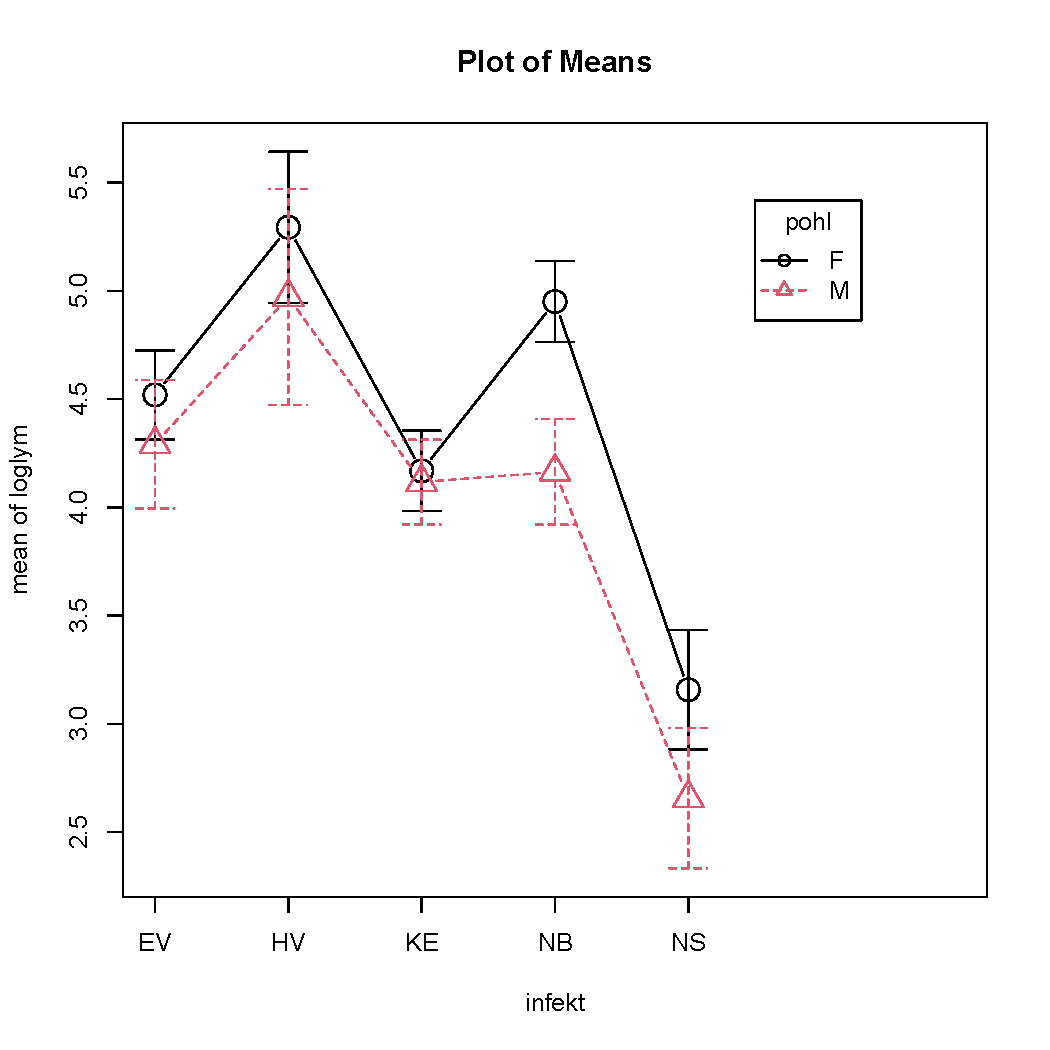
\includegraphics[width=\maxwidth]{figure/pr2-1} 
\begin{kframe}\begin{alltt}
\hlstd{mod2} \hlkwb{<-} \hlkwd{lm}\hlstd{(loglym} \hlopt{~} \hlstd{infekt} \hlopt{+} \hlstd{pohl,} \hlkwc{data}\hlstd{=lymfo,} \hlkwc{contrasts}\hlstd{=}\hlkwd{list}\hlstd{(}\hlkwc{infekt}\hlstd{=}\hlstr{"contr.Sum"}\hlstd{,}
  \hlkwc{pohl}\hlstd{=}\hlstr{"contr.Sum"}\hlstd{))}
\hlkwd{Anova}\hlstd{(mod2)}
\end{alltt}
\begin{verbatim}
## Anova Table (Type II tests)
## 
## Response: loglym
##            Sum Sq  Df F value    Pr(>F)    
## infekt     49.023   4  9.7121 4.247e-07 ***
## pohl        5.580   1  4.4218   0.03695 *  
## Residuals 214.524 170                      
## ---
## Signif. codes:  0 '***' 0.001 '**' 0.01 '*' 0.05 '.' 0.1 ' ' 1
\end{verbatim}
\begin{alltt}
\hlkwd{Tapply}\hlstd{(loglym} \hlopt{~} \hlstd{infekt} \hlopt{+} \hlstd{pohl, mean,} \hlkwc{na.action}\hlstd{=na.omit,} \hlkwc{data}\hlstd{=lymfo)} \hlcom{# means}
\end{alltt}
\begin{verbatim}
##       pohl
## infekt        F        M
##     EV 4.519428 4.291934
##     HV 5.293726 4.971128
##     KE 4.168507 4.116740
##     NB 4.950482 4.163947
##     NS 3.157443 2.657069
\end{verbatim}
\begin{alltt}
\hlkwd{Tapply}\hlstd{(loglym} \hlopt{~} \hlstd{infekt} \hlopt{+} \hlstd{pohl, sd,} \hlkwc{na.action}\hlstd{=na.omit,} \hlkwc{data}\hlstd{=lymfo)}
\end{alltt}
\begin{verbatim}
##       pohl
## infekt         F         M
##     EV 0.9400891 1.4548185
##     HV 1.3070840 1.4958171
##     KE 0.8694006 0.9608281
##     NB 0.8383912 1.2658070
##     NS 0.5508724 1.0763715
\end{verbatim}
\begin{alltt}
  \hlcom{# std. deviations}
\hlkwd{xtabs}\hlstd{(}\hlopt{~} \hlstd{infekt} \hlopt{+} \hlstd{pohl,} \hlkwc{data}\hlstd{=lymfo)} \hlcom{# counts}
\end{alltt}
\begin{verbatim}
##       pohl
## infekt  F  M
##     EV 21 24
##     HV 14  9
##     KE 22 24
##     NB 20 27
##     NS  4 11
\end{verbatim}
\end{kframe}
\end{knitrout}
Pomocí grafu plot of means můžeme vidět, že interakce mezi pohlavím a druhem infekce není, jen u klíšťová encefalitidy se průměry přibližují. I v modelu bez interakcí můžeme vidět, že oba faktory jsou signifikantní jsou menší než 0,05. Z toho lze usoudit, že pohlaví nijak neinteraguje s druhem infekce.

\end{document}
